\documentclass[envcountsect,envcountsame]{llncs}
%
\usepackage{makeidx}  % allows for indexgeneration
\usepackage{amsmath}
\usepackage{graphicx}
\usepackage{amssymb}
\usepackage{cite}
\usepackage{chngcntr}

%\bibliographystyle{plainurl}% the recommended bibstyle
\spnewtheorem{theorem1}{Theorem}{\bfseries}{\itshape}
\counterwithin{theorem1}{section}
\spnewtheorem{lem}[theorem1]{Lemma}{\bfseries}{\itshape}
\spnewtheorem{thm}[theorem1]{Theorem}{\bfseries}{\itshape}
\spnewtheorem{obs}[theorem1]{Observation}{\bfseries}{\itshape}
\spnewtheorem{cor}[theorem1]{Corollary}{\bfseries}{\itshape}


%\usepackage[noend, linesnumbered]{algorithm2e}
\usepackage{color}
\usepackage{cite}
\usepackage{pifont}
\usepackage{xspace}
\usepackage{enumerate}
\usepackage{tikz}
\usetikzlibrary{calc, shapes, backgrounds, trees, decorations.pathmorphing,
decorations.markings, decorations.pathreplacing, positioning, patterns}


\newcommand\polylog{{\rm polylog}}
\newcommand\A{{\mathcal A}}
\newcommand\B{{\mathcal B}}
\newcommand\C{{\mathcal C}}
\newcommand\DC{{\mathcal D}}
\newcommand\E{\mathbf{E}}
\newcommand\F{{\mathcal F}}
\newcommand\G{{\mathcal G}}
\def\L{{\mathcal L}}
\def\K{{\mathcal K}}
\def\M{{\mathcal M}}
\def\N{{\mathbb N}}
\def\P{{\mathcal P}}
\def\Q{{\mathcal Q}}
\def\cR{{\mathcal R}}
%\def\S{{\mathcal S}}
\def\U{{\mathcal U}}
\def\T{{\mathcal T}}
\def\W{{\mathcal W}}
\def\V{{\mathcal V}}
\def\Z{{\mathbb Z}}
\def\etal{\emph{et~al.}\xspace}
\def\DD{{\small \Delta}}
\def\bd{{\partial}}
\newcommand{\bigO}{\mathcal{O}}
\newcommand{\tmin}{T_{\min}} % runtime of the minimal element
\newcommand{\pre}{{pre}}
\newcommand{\lcp}{\operatorname{lcp}} % longest common prefix
\newcommand{\searchI}{\textit{search}_{I}}
\newcommand{\searchIDefinition}{\searchI(q) = \max\{\alpha \in \pre(q) \mid
T[\alpha] \not= \bot\}}
\newcommand{\smallO}{{o}}
\newcommand{\bigW}{{\Omega}}
\newcommand{\lca}{\operatorname{lca}} % longest common ancestor


%\usepackage{subcaption}


\def\aa{{\bf a}}
\def\bb{{\bf b}}
\def\hh{{\bf h}}
\def\kk{{\bf k}}
\def\pp{{\bf p}}
\def\qq{{\bf q}}
\def\xx{{\bf x}}
\def\yy{{\bf y}}
\def\uu{{\bf u}}
\def\vv{{\bf v}}
\def\ww{{\bf w}}

\DeclareMathOperator{\NN}{NN}
\DeclareMathOperator{\D}{D}


\newcommand{\mathset}[1]{\ensuremath {\mathbb {#1}}}
\newcommand{\eps}{\varepsilon}
\newcommand{\R}{\mathset{R}}
\newcommand{\script}[1]{\ensuremath {\mathcal {#1}}}
\setlength{\fboxsep}{.5pt}
\newcommand{\mc}{\mathcal}
%\renewcommand\thefootnote{\tiny\protect\framebox{\arabic{footnote}}}
\newcommand{\abs}[1]{\left\lvert#1\right\rvert}


\newcommand{\remarkcmd}[3]{\textcolor{blue}{\textsc{#1 #2:}}
  \textcolor{red}{\textsf{#3}}}
\newcommand{\marcel}[2][says]{\remarkcmd{Marcel}{#1}{#2}}
\newcommand{\wolfgang}[2][says]{\remarkcmd{Wolfgang}{#1}{#2}}

%------------------------------ Text -------------------------------------
\usepackage{amsmath,amssymb}
\let\doendproof\endproof
\renewcommand\endproof{~\hfill\qed\doendproof}


\begin{document}
%
\frontmatter          % for the preliminaries
%
\pagestyle{headings}  % switches on printing of running heads

\mainmatter   
%
\title{Delta-Fast Tries: Local Searches in Bounded Universes
with Linear Space\thanks{Supported in part by 
DFG project MU/3501-1.}}
%
\titlerunning{Delta-Fast Tries}  % abbreviated title (for running head)
%
\author{Marcel Ehrhardt \and Wolfgang Mulzer}
%
\authorrunning{Marcel Ehrhardt and Wolfgang Mulzer} % abbreviated author list (for running head)
%
\institute{
Institut f\"ur Informatik, Freie Universit\"at Berlin, Germany\\
\email{[marehr,mulzer]@inf.fu-berlin.de}
}
%
\maketitle  
\begin{abstract}
Let $w \in \N$ and $U = \{0, 1, \dots, 2^w-1\}$ be a 
bounded universe of $w$-bit integers.  We present a 
dynamic data structure for predecessor searching in 
$U$.  Our structure needs $O(\log \log \Delta)$ time 
for queries and $O(\log \log \Delta)$ expected time 
for updates, where $\Delta$ is the difference between 
the query element and its nearest neighbor in the 
structure. Our data structure requires linear space. 
This improves a result by Bose~\etal [CGTA, 46(2), pp.~181--189].

The structure can be applied for answering approximate nearest
neighbor queries in low dimensions and for dominance queries on
a grid.
\end{abstract}

\section{Introduction}

Predecessor searching is one of the oldest problems in 
theoretical computer science~\cite{CormenLeRiSt09,Knuth98}.
Let $U$ be a totally ordered universe. The task
is to maintain a set $S \subseteq U$,
while supporting
\emph{predecessor} and \emph{successor} queries: 
given $q \in U$, find the largest element in $S$ 
smaller than $q$ ($q$'s predecessor) or the 
smallest element in $S$ larger than $q$
($q$'s successor). In the \emph{dynamic}
version of the problem, we also want to 
be able to modify $S$ by inserting and/or 
deleting elements.

In the \emph{word-RAM } model of computation,
all input elements are $w$-bit words, where
$w \in \N$ is a parameter. Without loss of 
generality, we may assume that $w$ is a power 
of $2$. We are allowed to manipulate the input 
elements at the bit level, in constant time per 
operation. In this case, we may assume that the 
universe is $U = \{0, \dots, 2^{w}-1\}$. 
A classic solution for predecessor searching on the
word-RAM is due to van Emde Boas, who
described a dynamic data structure that
requires space $O(n)$ and supports insertions,
deletions, and predecessor queries in $O(\log\log |U|)$ 
time~\cite{vEmdeBoas77,vEmdeBoasKaZi76}.

In 2013, Bose~\etal~\cite{BoseDoDuHoMo13} described
a word-RAM data structure for the predecessor
problem that is \emph{local} in the following sense.
Suppose our data structure currently contains the
set $S \subseteq U$, and let $q \in U$ be a query
element.  Let $q^+ := \min\{s \in S \mid s \geq q \}$ and
$q^- := \max\{s \in S \mid s \leq q \}$ be the 
successor and the predecessor of $q$ in $S$, and let
$\Delta= \min\{|q- q^-|, |q-q^+|\}$ be the distance
between $q$ and its nearest neighbor in $S$. Then, 
the structure by Bose \etal can answer predecessor 
and successor queries in $O(\log\log \Delta)$ time.
Their solution requires $\bigO(n \log\log\log|U|)$ words 
of space, where $n = |S|$ is the size of the 
current set. Bose~\etal apply their structure 
to obtain a fast data structure for approximate nearest 
neighbor queries in low dimensions and for answering
dominance and range searching queries on a grid.

Here, we show how to obtain a data structure with similar
guarantees for the query and update times that reduces the
space requirement to $O(n)$. This solves an open problem 
from~\cite{BoseDoDuHoMo13}. Furthermore,  this also improves the space 
requirement for data structures for nearest neighbor searching
and dominance reporting.
Full details and pseudocode for all the algorithms and
data structures described here can 
be found in the Master's thesis of the first author~\cite{Ehrhardt15}.
Belazzougui~\etal give a linear space bound for distance-sensitive
queries in the static setting, using almost the same 
techniques as in the present paper~\cite{BelazzougiBoVi12}. Our 
result was obtained independently from the work of 
Belazzougui~\etal

\section{Preliminaries}
\label{sec:prelim}

We begin by listing some known structures and background information
required for our data structure.

\paragraph{Compressed Tries.}
Our data structure is based on \emph{compressed
tries}~\cite{CormenLeRiSt09}. These are defined as
follows: we interpret the elements from $S$ as bitstrings 
of length $w$ (the most significant bit being in the leftmost
position). The \emph{trie} $T'$ for $S$ is a binary tree
of height $w$. Each node $v \in T'$ corresponds
to a bitstring $p_v \in \{0,1\}^*$. The root $r$ has
$p_r = \eps$. For each inner node $v$, the left
child $u$ of $v$  has $p_u = p_v0$, and the
right child $w$ of $v$ has $p_w = p_v1$ (one of the
two children may not exist). The bitstrings of the 
leaves correspond to the elements of $S$, and
the bitstrings of the inner nodes are prefixes
for the elements in $S$, see Figure~\ref{fig:trie}.

\begin{figure}
  \centering
  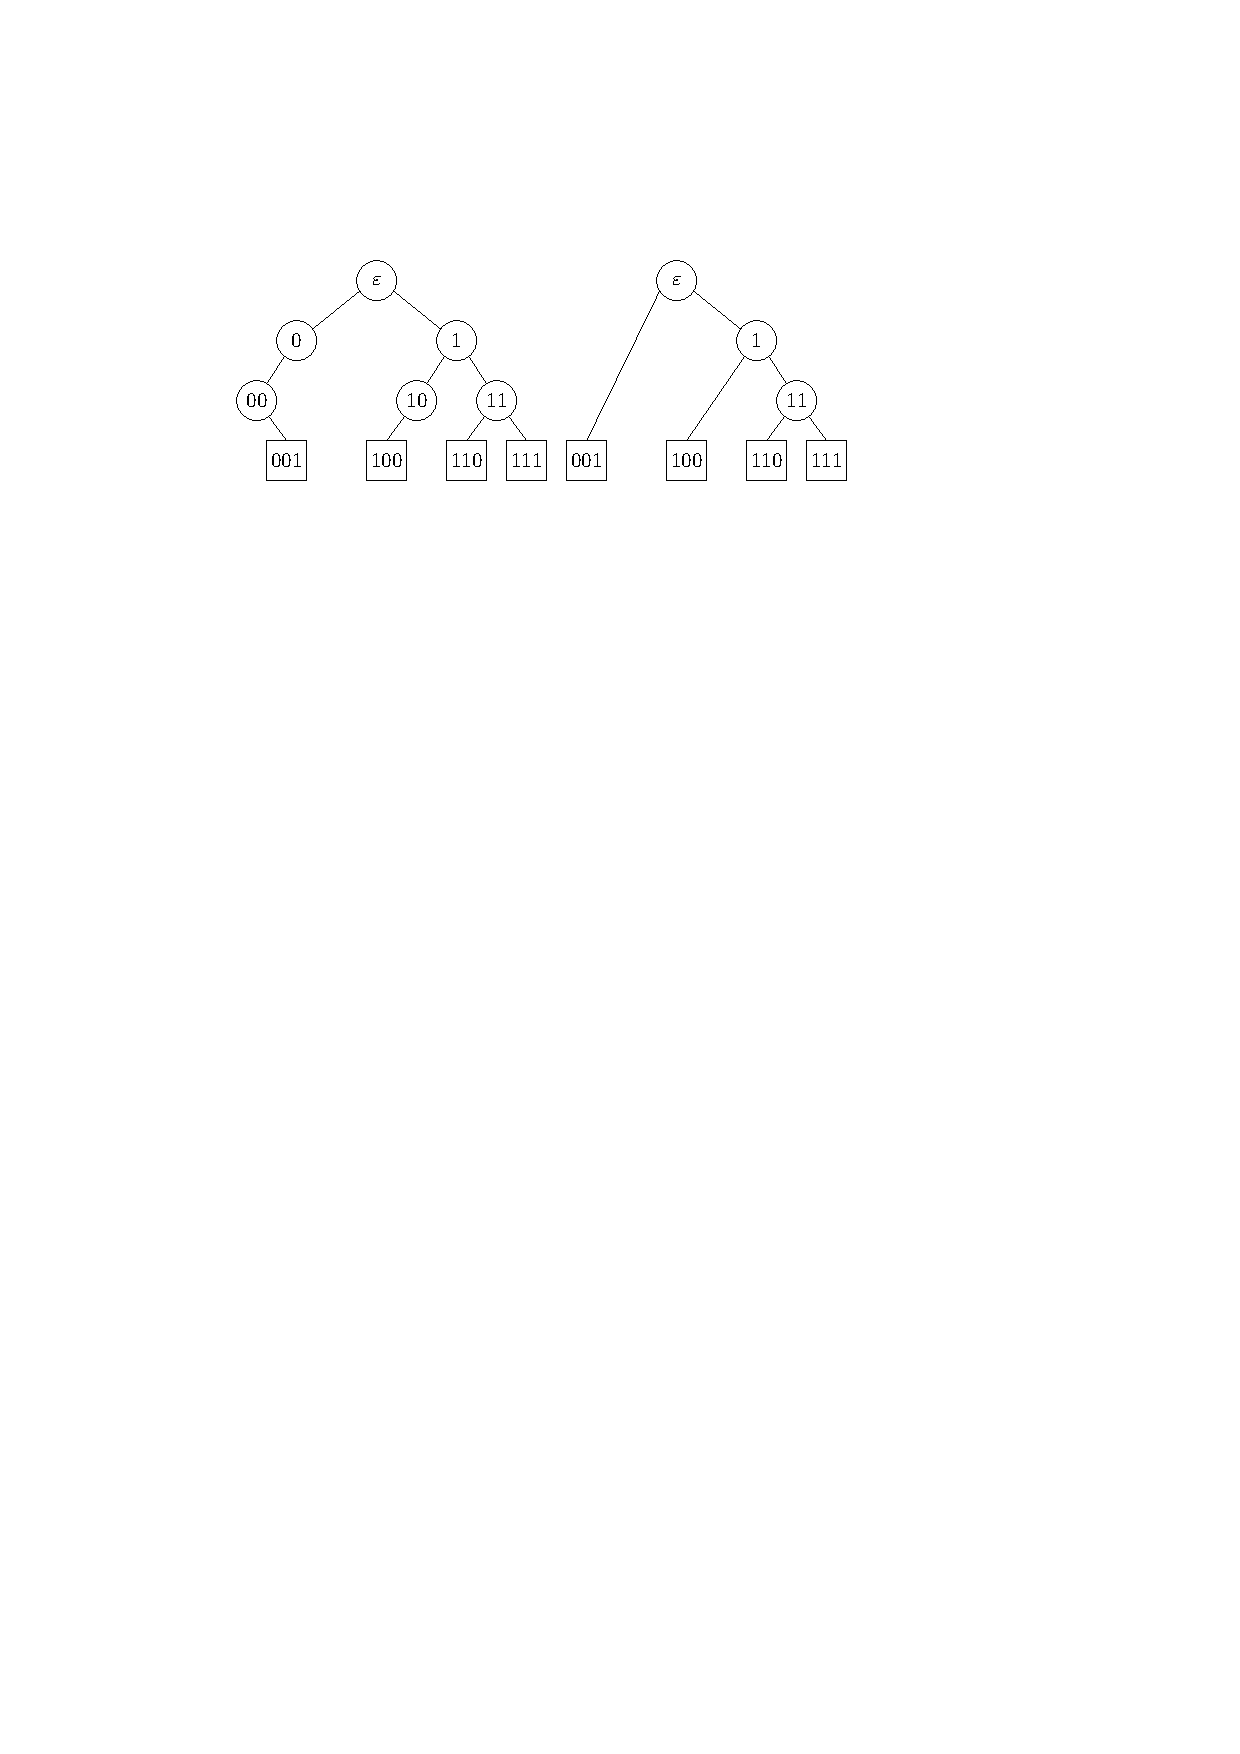
\includegraphics{img/trie}
  \caption{A trie (left) and a compressed trie (right) for the set 
  000, 100, 110, 111. The longest common prefix of 101 is  10. The 
  lca of 101 in the compressed trie
    is the node labeled 1.}
  \label{fig:trie}
\end{figure}

The \emph{compressed trie} $T$ for $S$ is obtained
from $T'$ by contracting each maximal path of nodes
with only one child into a single edge. 
Each inner node in $T$ has exactly two children, and
consequently $T$ has $O(n)$ nodes.
Maybe somewhat unusually, in the following, the 
\emph{height} and \emph{depth} of a node $v$ in $T$ 
will refer to the corresponding
height and depth in the (uncompressed) trie $T'$.
This convention will make the description of the operations more
convenient.

Let $q \in \{0,1\}^*$ be a bitstring of length at most $w$.
The \emph{longest common prefix} of $q$ with $S$, $\lcp_S(q)$,
is the longest prefix that $q$ shares with an element 
in $S$. We say that $q$ \emph{lies on an edge}
$e = (u, v)$ of $T$ if $p_u$ is a prefix of $q$ and
$q$ is a proper prefix of $p_v$. If $\lcp_S(q)$
lies on the 
edge $(u,v)$, we call $u$ the \emph{lowest common
ancestor} of $q$ in $T$, denoted by
$\lca_T(q)$. One can show that $\lca_T(q)$ is uniquely
defined.

\paragraph{Associated Keys.}
Our algorithm uses the notion of
\emph{associated keys}. This notion
was introduced in the context of 
\emph{$z$-fast tries}~\cite{BelazzouguiBoVi10,Ruzic09},
and it is also useful in our data structure.

Associated keys provide a quick way to compute $\lca_T(q)$,
for any element $q \in U$.
A natural way to find $\lca_T(q)$ is
to do binary search on the depth of $\lca_T(q)$:
we initialize $(l,r) = (0,w)$ and let 
$m = (l+r)/2$. We denote by $q' = q_0\dots q_{m-1}$ 
the leftmost $m$ bits of $q$, and we check whether
$T$ has an edge $e = (u,v)$ such that $q'$ lies on $e$.
If not, we set $r = m$, and we continue.
Otherwise, we determine if $u$ is $\lca_T(q)$, by
testing whether $p_v$ is not a prefix of $q$.
If $u$ is not $\lca_T(q)$, we set $l = m$ and continue.
In order to perform this search quickly,
we need to find the edge $e$ that
contains a given prefix $q'$, if it exists. For this,
we precompute for each edge $e$ of $T$
the first time that the binary search
encounters a prefix that lies on $e$. This
prefix is uniquely determined and depends only on 
$e$, not on the specific string $q$ that we are looking 
for. We let $\alpha_e$ be
this prefix, and we call $\alpha_e$ the \emph{associated key}
for $e = (u,v)$, see Figure~\ref{fig:binsearch}. 
\begin{figure}
\centering
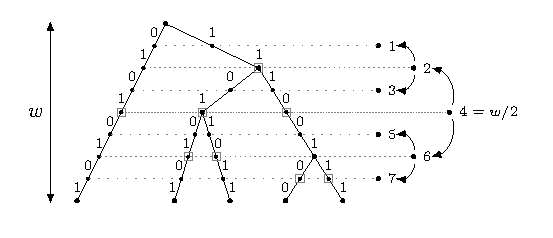
\includegraphics{img/binsearch_assoc_key_main}
\caption{The associated key $\alpha_e$ of an edge $e$:
we perform a binary search on the height of
$\lcp_S(q)$ in $T$. The \emph{associated key}
of an edge $e$ is the prefix of $\lcp_S(q)$ in which the
search first encounters the edge $e$. }
\label{fig:binsearch}
\end{figure}


The binary search needs $\log w$ steps, and 
since we assumed that $w$ is a power of two,
each step determines the next bit in the binary 
expansion of the \emph{length} of $\lcp_S(q)$.
Thus, the associated key of an edge $e$
can be computed in $O(1)$ time on a word RAM 
as follows: consider the $\log w$-bit binary 
expansions $\ell_u = |p_u|_2$ and  $\ell_v = |p_v|_2$ of the
\emph{lengths} of the prefixes
$p_u$ and $p_v$, and let $\ell'$ be the
longest common prefix of $\ell_u$ and
$\ell_v$. We need to determine the first
step when the binary search can distinguish between
$\ell_u$ and $\ell_v$. Since $\ell_u < \ell_v$,
and since the two binary expansions differ in the
first bit after $\ell'$,
it follows that $\ell_u$ begins with $\ell'0$ and
$\ell_v$ begins with $\ell'1$. Thus, let $\ell$ be obtained
by taking $\ell'$, followed by $1$ and
enough $0$'s to make a $\log w$-bit
word. Let $l$ be the number encoded by $\ell$.
Then, the associated key $\alpha_e$ consists of the 
first $l$ bits of $p_v$;
see~\cite{BelazzouguiBoVi10,Ehrhardt15,Ruzic09} for more details.

\paragraph{Hash Maps.}
Our data structure also makes extensive use of
hashing. In particular, we will maintain several
succinct hashtables that store additional
information for supporting fast queries.
For this, we will use a hashtable described
by Demaine~\etal~\cite{DemaineMePaPa06}.
The following theorem summarizes the properties
of their data structure.

\begin{theorem}\label{thm:succinct_retrieval_only_hashtable}
For any $r \geq 1$, there exists a dynamic dictionary that
stores entries with keys from $U$ and with associated
values of $r$ bits each.
The dictionary supports updates and queries in $O(1)$ time,
using $O(n \log\log (|U|/n) + nr)$ \emph{bits} of space.
The bounds for the space and the queries are
worst-case, the bounds for the updates hold with
high probability.\qed
\end{theorem}

\section{Static $\Delta$-fast Tries}
\label{sect:delta-fast_trie}

We are now ready to describe our data structure 
for the static case. In the next section, we will
discuss how to add support for insertions and
deletions.

\subsection{The Data Structure}
Our data structure is organized as follows:
let $S \subseteq U$, $|S| = n$, be given.
We store $S$ in a compressed trie
$T$. The leaves of $T$ are
linked in sorted order. Furthermore, 
for each node $v$ of $T$, let $T_v$ be the
subtree rooted at $v$. Then, $v$ stores pointers 
to the smallest and the largest leaf in 
$T_v$. To support the queries, we store 
three additional hash maps: $H_\Delta$, $H_z$,
and $H_b$.

First, we describe the hash map $H_\Delta$.
Set $m = \log\log w$. For
$i = 0, \dots, m$, we let
$h_i = 2^{2^i}$ and  
$d_i = w - h_i$. 
The hash map $H_\Delta$ stores the following
information: for each $s \in S$ and each
$d_i$, $i = 1, \dots, m$,
let $s_i = s_0 \dots s_{d_i-1}$ be the leftmost
$d_i$-bits of $s$ and let $e = (u,v)$ be
the edge of $T$ such that $s_i$ lies
on $e$.
Then, $H_\Delta$ stores the entry
$s_i \mapsto u$.

Next, we describe the hash map $H_z$.
It is defined similarly as the hash map
used for $z$-fast tries~\cite{BelazzouguiBoVi10,Ruzic09}.
For each edge $e$ of $T$, let $\alpha_e$ be
the associated key of $e$, as explained in 
Section~\ref{sec:prelim}.
Then, $H_z$ stores the entry $\alpha_e \mapsto e$.


Finally, the hash map $H_b$ is used to implement
a second layer of indirection that lets us achieve
linear space. It will be described below.

\subsection{The Predecessor Query}
\label{sec:staticquery}

Let $q \in U$ be the query, and let
$q^-$ and $q^+$ be the predecessor and
the successor of $q$ in $S$, as described above.
We first show how to get a running time
of $O(\log\log \Delta)$ for the queries, with  
$\Delta = |q - q^+|$.  In Theorem~\ref{thm:staticresult}, we will 
see that this can easily be improved
to $\Delta = \min\{|q - q^-|, |q - q^+|\}$.

The predecessor search works in several 
\emph{iterations}. In iteration $i$, we consider
the prefix $q_i$ that consists of the first $d_i$ 
bits of $q$.

First, we check whether 
$H_\Delta$ contains an entry for
$q_i$. If so, we know that $T$ contains
an edge $e$ such that $q_i$ lies on $e$.
Hence, $q_i$ must be  a prefix of $\lcp_S(q)$.
If one of the endpoints of $e$ happens to be
$\lca_T(q)$, we are done.
Otherwise, we consider the two edges emanating from  the lower
endpoint of $e$, finding the edge $e'$ that lies on
the path to $q$.
We take the associated key $\alpha_{e'}$ of $e'$,
and we use it to continue the binary search
for $\lca_T(q)$, as described in
Section~\ref{sec:prelim}. Since $|q_i| = d_i$,
this binary search takes 
$O(\log (w - d_i)) = O(\log h_i)$ steps to complete.
Once the lowest common ancestor $v = \lca_T(q)$ is 
at hand,  we can find the predecessor of $q$ in $O(1)$ 
additional time: it is either the rightmost element in $T_v$,
the predecessor of the leftmost element in $T_v$, or the 
rightmost element in the left subtree of $v$. Given the 
pointers stored with $v$ and the leaves of $T$, all these
nodes can be found in $O(1)$ time.

If $H_\Delta$ contains no entry for
$q_i$ and if $q_i$ does not consist
of all $1$'s, we check if $H_\Delta$ contains
an entry for $q_i + 1$.
Notice that $q_i+1$ is the successor of $q_i$. 
If such an entry exists,
we first obtain $u = H_\Delta[q_i +1]$, and the child $v$ of 
$u$ such that $q_i + 1$ lies on the edge $e = (u,v)$.
Then, we follow the pointer to the leftmost element of
$T_v$. This is the successor $q^+$ of $q$. 
The predecessor $q^-$ can then be found by following the 
leaf pointers. This takes $O(1)$ time overall.

Finally, if there is neither an entry for $q_i$
nor for $q_i+1$, we continue 
with iteration $i+1$, see Figure~\ref{fig:query}.

\begin{figure}
\centering
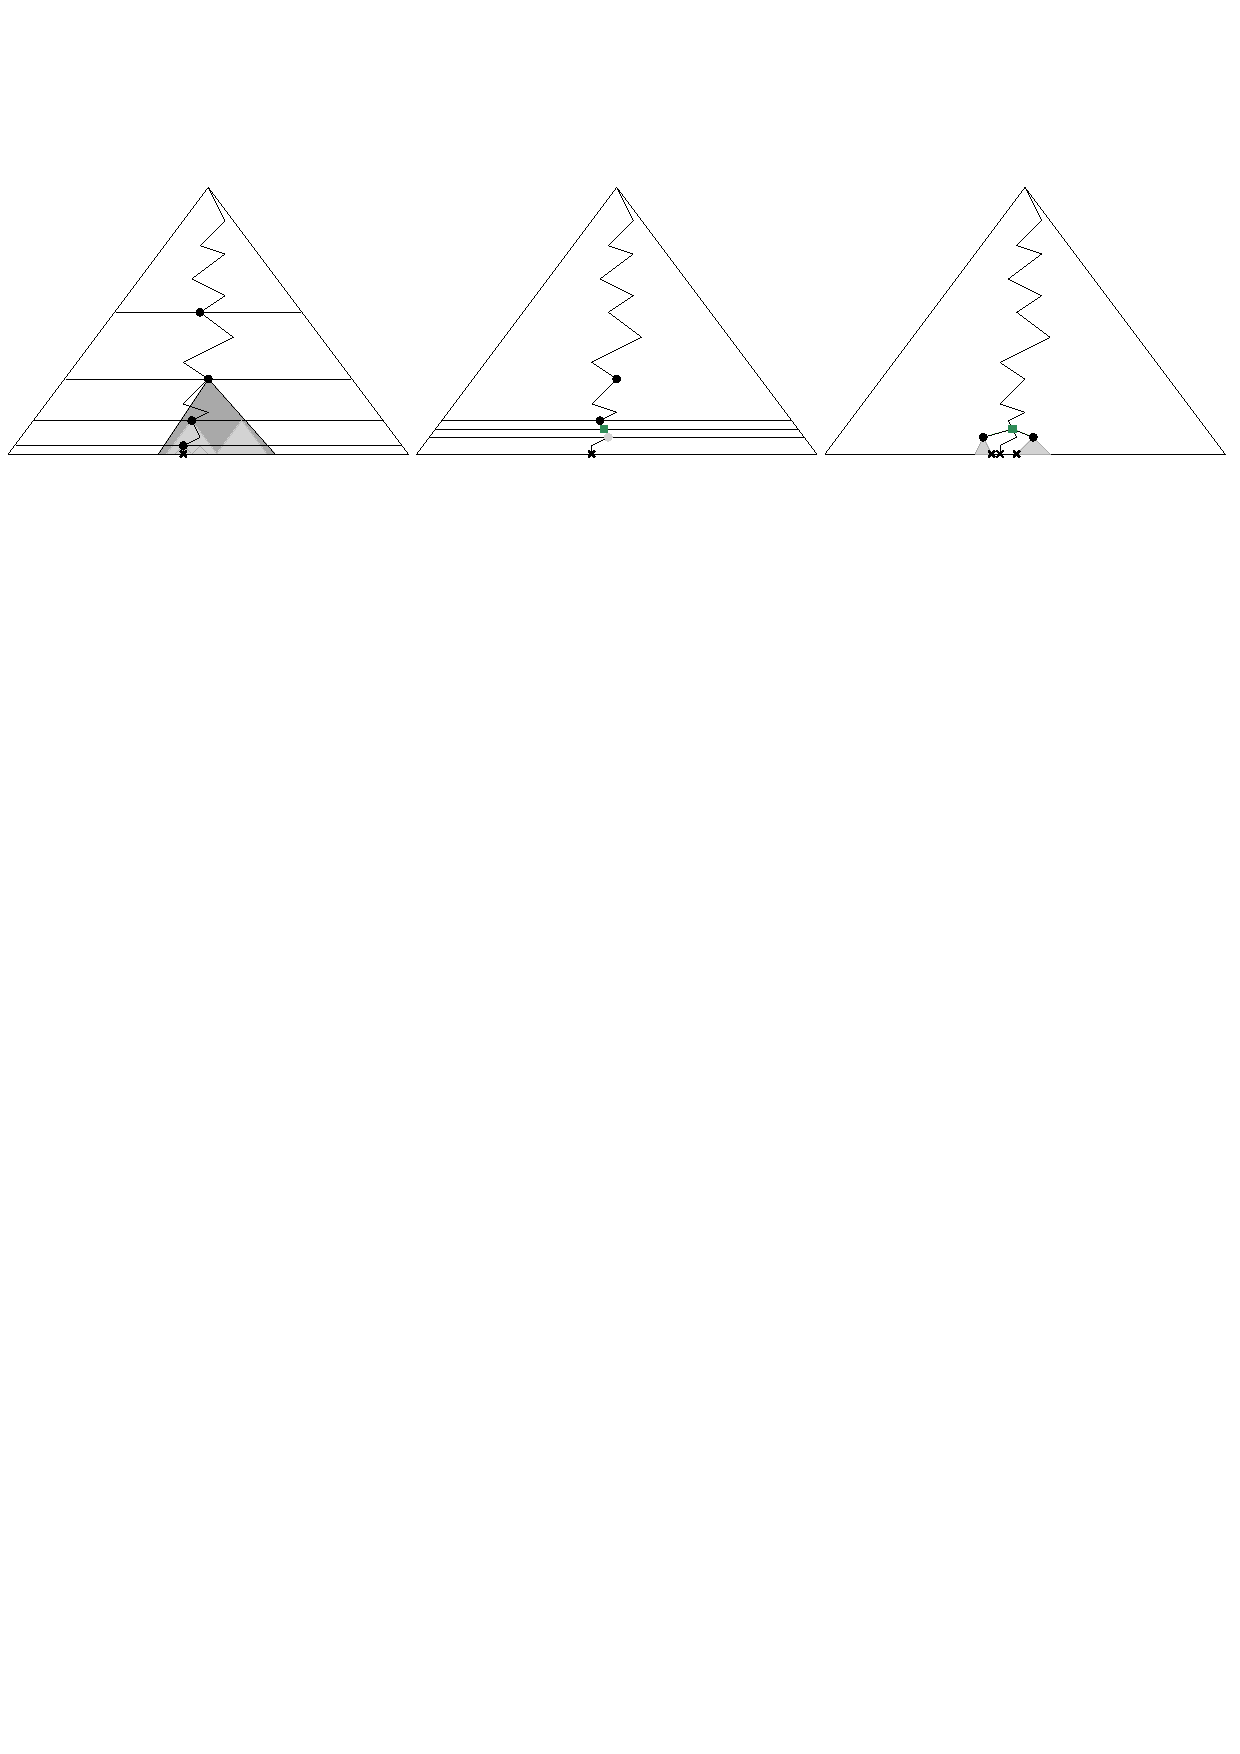
\includegraphics[scale=0.5]{img/query}
\caption{The query algorithm: first we perform an
exponential search from the lowest level, to find a prefix
of $q_k$  or $q_k+1$ (left). If a prefix $q_{k}$ is found,
we perform a binary search for $\lca_T(q)$ (middle), which can then
be used to find the predecessor and successor of $q$ (right). If
a prefix $q_k+1$ is found, the successor and predecessor 
can be found immediately (not shown).}
\label{fig:query}
\end{figure}

From the above discussion, it follows that
the total time for the predecessor
query is $O(k + \log h_k)$, where $k$ is the number of 
iterations and $\log h_k$ is the worst-case time 
for the predecessor search once one of the lookups 
in an iteration succeeds. 
By our predecessor algorithm, we know that $S$ contains no element with
prefix $q_{k-1}$ or $q_{k-1} + 1$, but an element with
prefix $q_k$ or $q_k + 1$. Thus, there must be
at least $2^{w - d_k} = 2^{h_k}$ consecutive elements in 
$U\setminus S$ following $q$. By our definition of $h_k$, it follows that
$\Delta \geq 2^{h_{k-1}} = 2^{2^{2^{k-1}}}$, so 
$k \leq 1 + \log\log\log \Delta$.
Furthermore, since $h_k = 2^{2^k} = \left(2^{2^{k-1}}\right)^2 
=  (h_{k-1})^2$, 
it follows that $h_k = O(\log^{2} \Delta)$.

\subsection{Obtaining Linear Space}
We now analyze the space requirement for our
data structure.
Clearly,  the  trie $T$ and the
hash map $H_z$ require $O(n)$ words of space.
Furthermore, as described so far, the number of 
words needed for
$H_\Delta$ is $O(n \log\log w)$, since 
we store at most $n$ entries for each 
height $h_i$, $i = 0, \dots, m = \log\log w$.

Using a trick due to P\v{a}tra\c{s}cu~\cite{Patrascu10}, 
we can introduce another level of indirection to reduce 
the space requirement to  $O(n)$.
The idea is to store in $H_\Delta$ the \emph{depth}
$d_u$ of each branch node $u$ in $T_\Delta$, instead of storing 
$u$ itself (here, we mean the depth in the
original trie, i.e., the length of the prefix $p_u$). 
We then use an additional hash map 
$H_b$ to obtain $u$.
This is done as follows:
when trying to find the branch node $u$ for a given
prefix $q_i$, we 
first get the depth $d_u = |p_u|$ of $u$ 
from $H_\Delta$. After that, we look up the branch
node $u = H_b[q_0 \dots q_{d_u-1}]$ from the hash map 
$H_b$. Finally, we check whether $u$ is actually the 
lowest branch node of $q_i$. If any of those steps fails,
we return $\bot$.

Let us analyze the needed space: clearly, $H_b$ needs
$O(n)$ words, since it stores $O(n)$ entries.
Furthermore,
we have to store $O(n \log\log w)$ entries in 
$H_\Delta$, each mapping a prefix $q_i$ to the depth of 
its lowest branch node. This depth requires
$\lceil \log w \rceil$ bits.
By Theorem~\ref{thm:succinct_retrieval_only_hashtable},
a retrieval only hash map for $n'$ items and $r$ bits 
of data needs $O(n'\log\log \frac{|U|}{n'} + n'r)$ bits.
Therefore, the space 
\emph{in bits} for $H_\Delta$ is proportional to
\begin{align*}
&\phantom{=} n \log\log w \cdot \log\log \frac{|U|}{n \log\log w} +
n \log\log w \cdot \lceil \log w \rceil\\
&= O(n \log\log w \cdot \log w)\\
&= o(n\cdot w),
\end{align*}
using $n' = n\log\log w$, $r = \lceil \log w \rceil$ and $w = \log |U|$. 
Thus, we can store $H_\Delta$ in 
$O(n)$ words of $w$ bits each. The following lemma summarizes
the discussion

\begin{lemma}
\label{lemma:delta_linear_space}
The $\Delta$-fast trie needs $O(n)$ words space.
\end{lemma}

\subsection{Putting it Together}

We can now obtain our result for the static predecessor problem.

\begin{theorem}\label{thm:staticresult}
Let $U = \{0, \dots, 2^{w}-1\}$ and let
$S \subseteq U$, $|S| = n$.
The static $\Delta$-fast trie for $S$ requires
$O(n)$ words of space, and it can answer
a static predecessor query for an element $q \in U$ on $S$ in time
$O(\log \log \min\{|q-q^-|, |q-q^+|\})$,
where $q^-$ and $q^+$ denote the predecessor
and successor of $q$ in $S$.
The preprocessing time is 
$O(n \log\log \log |U|)$, assuming that
$S$ is sorted.
\end{theorem}

\begin{proof}
The regular search for $q \in S$ can be done in 
$O(1)$ time by a lookup in $H_z$. 
We have seen that the predecessor of $q$
can be found in $O(\log \log |q-q^+|)$ time.
A symmetric result also holds for 
successor queries.
In particular, we can achieve query time 
$O(\log \log |q-q^-|)$  by checking for
$H_\Delta[q_i-1]$ instead of $H_\Delta[q_i+1]$ in the 
query algorithm. 

By interleaving the two searches,
we obtain the desired running time of 
$O(\log\log \min\{|q - q^-|, |q - q^+|\})$. 
Of course, in a practical implementation, it would be 
more efficient to check directly for $H_\Delta[q_i-1]$
and $H_\Delta[q_i+1]$ in the query algorithm.

The trie $T$ and the hash maps $H_z$
and $H_b$ can be computed in $O(n)$ time, given that
$S$ is sorted.
Thus, the preprocessing time is dominated by the time to fill the 
hash map $H_\Delta$.  Hence, the preprocessing needs
$O(n\log\log\log |U|)$ steps, because $\bigO(n\log\log w)$ nodes 
have to be
inserted into $H_\Delta$. 
By Lemma~\ref{lemma:delta_linear_space}, the space requirement
is linear.
\end{proof}

\section{Dynamic $\Delta$-fast tries}

We will now explain how to extend our data
structure to the dynamic case. 
The basic data structure remains the same, but
we need to update the hashtables and the trie $T$
after each insertion and deletion.
In particular, our data structure requires that
for each $v$ in $T_v$, we can access the 
leftmost and the rightmost node
in the subtree $T_v$.
In the static case, this could be done simply
by maintaining explicit pointers from each node
$v \in T$ to these nodes in $T_v$, letting us find
the nodes in $O(1)$ time.
In the dynamic case, we will maintain a data structure
which allows finding and updating these nodes in
in $O(\log\log \Delta)$ time.

\subsection{Computing Lowest Common Ancestor}

To perform the update operation, we need a
procedure to compute the lowest common ancestor 
$\lca_T(q)$ for any given element $q \in U$. 
For this, we proceed as in the query algorithm from 
Section~\ref{sec:staticquery}, but skipping 
the lookups for $H_\Delta[q_i-1]$ and
$H_\Delta[q_i+1]$. By the analysis in 
Section~\ref{sec:staticquery}, this will find 
$\lca_T(q)$ in time $O(\log \log l)$, where $l$
is height of $\lca_T(q)$ in $T$.

Unfortunately, it may happen that this height $l$ is as large as $w$,
even if $q$ is close to an element in the current set $S$.
To get around this, we use a trick of Bose~\etal~\cite{BoseDoDuHoMo13}.
Namely, their idea is to perform a random shift of the universe. 
More precisely, we pick a random number $r \in U$, and we
add $r$ to all query and update elements that appear in 
the data structure (modulo $|U|$).

\begin{lemma}[Lemma 4 in \cite{BoseDoDuHoMo13}]
\label{lemma:delta_lca_loglog_delta}
Let $x, y \in U$ be two fixed elements in $U$.
Let $r \in U$ be picked uniformly at random.
After a random shift of $U$ by $r$, the 
expected height of the lowest common ancestor of 
$x$ and $y$ in a compressed trie is $O(\log|x-y|)$.\qed
\end{lemma}

\begin{cor}
\label{cor:delta_fast_expected_lca}
Let $S \subseteq U$ and let $T$ be a randomly
shifted $\Delta$-fast trie storing $S$.
Let $q \in U$. 
We can find $\lca_T(q)$ in expected time $O(\log\log \Delta)$,
where $\Delta = \min\{|q - q^+|, |q-q^-|\}$, the elements 
$q^+$ and $q^-$ being the predecessor and successor of $q$ in $S$.
The expectation is
over the random choice of the shift $r$. 
\end{cor}

\begin{proof}
Suppose without loss of generality that $\Delta = |q - q^+|$.
By Lemma~\ref{lemma:delta_lca_loglog_delta},
the expected height $h_k$ of the lowest common ancestor of $q$ and $q^+$
is $O(\log \Delta)$.
We perform the doubly exponential
search on the prefixes of $q$, as in Section~\ref{sec:staticquery} 
(without checking $q_i+1$) to find the height $h_k$. After
that, we  resume the search for $\lca_T(q)$ on the 
remaining $h_k$ bits. Since $h_k = O(\log \Delta)$ in expectation,
it follows by Jensen's inequality that the number $k$
of loop iterations to find  $h_k$ is $O(\log\log\log \Delta)$
in expectation. Thus, the expected running time is proportional to
$k + \log h_k = O(\log\log\Delta)$. 
\end{proof}

\subsection{Managing the Left- and Rightmost Elements 
of the Subtrees}

We also need to maintain for each node $v \in T$ the
leftmost and the rightmost element in the subtree $T_v$.
In the static case, it suffices to have direct pointers
from $v$ to the respective leaves, but
in the dynamic case, we need an additional data structure. 

\begin{figure}
\centering
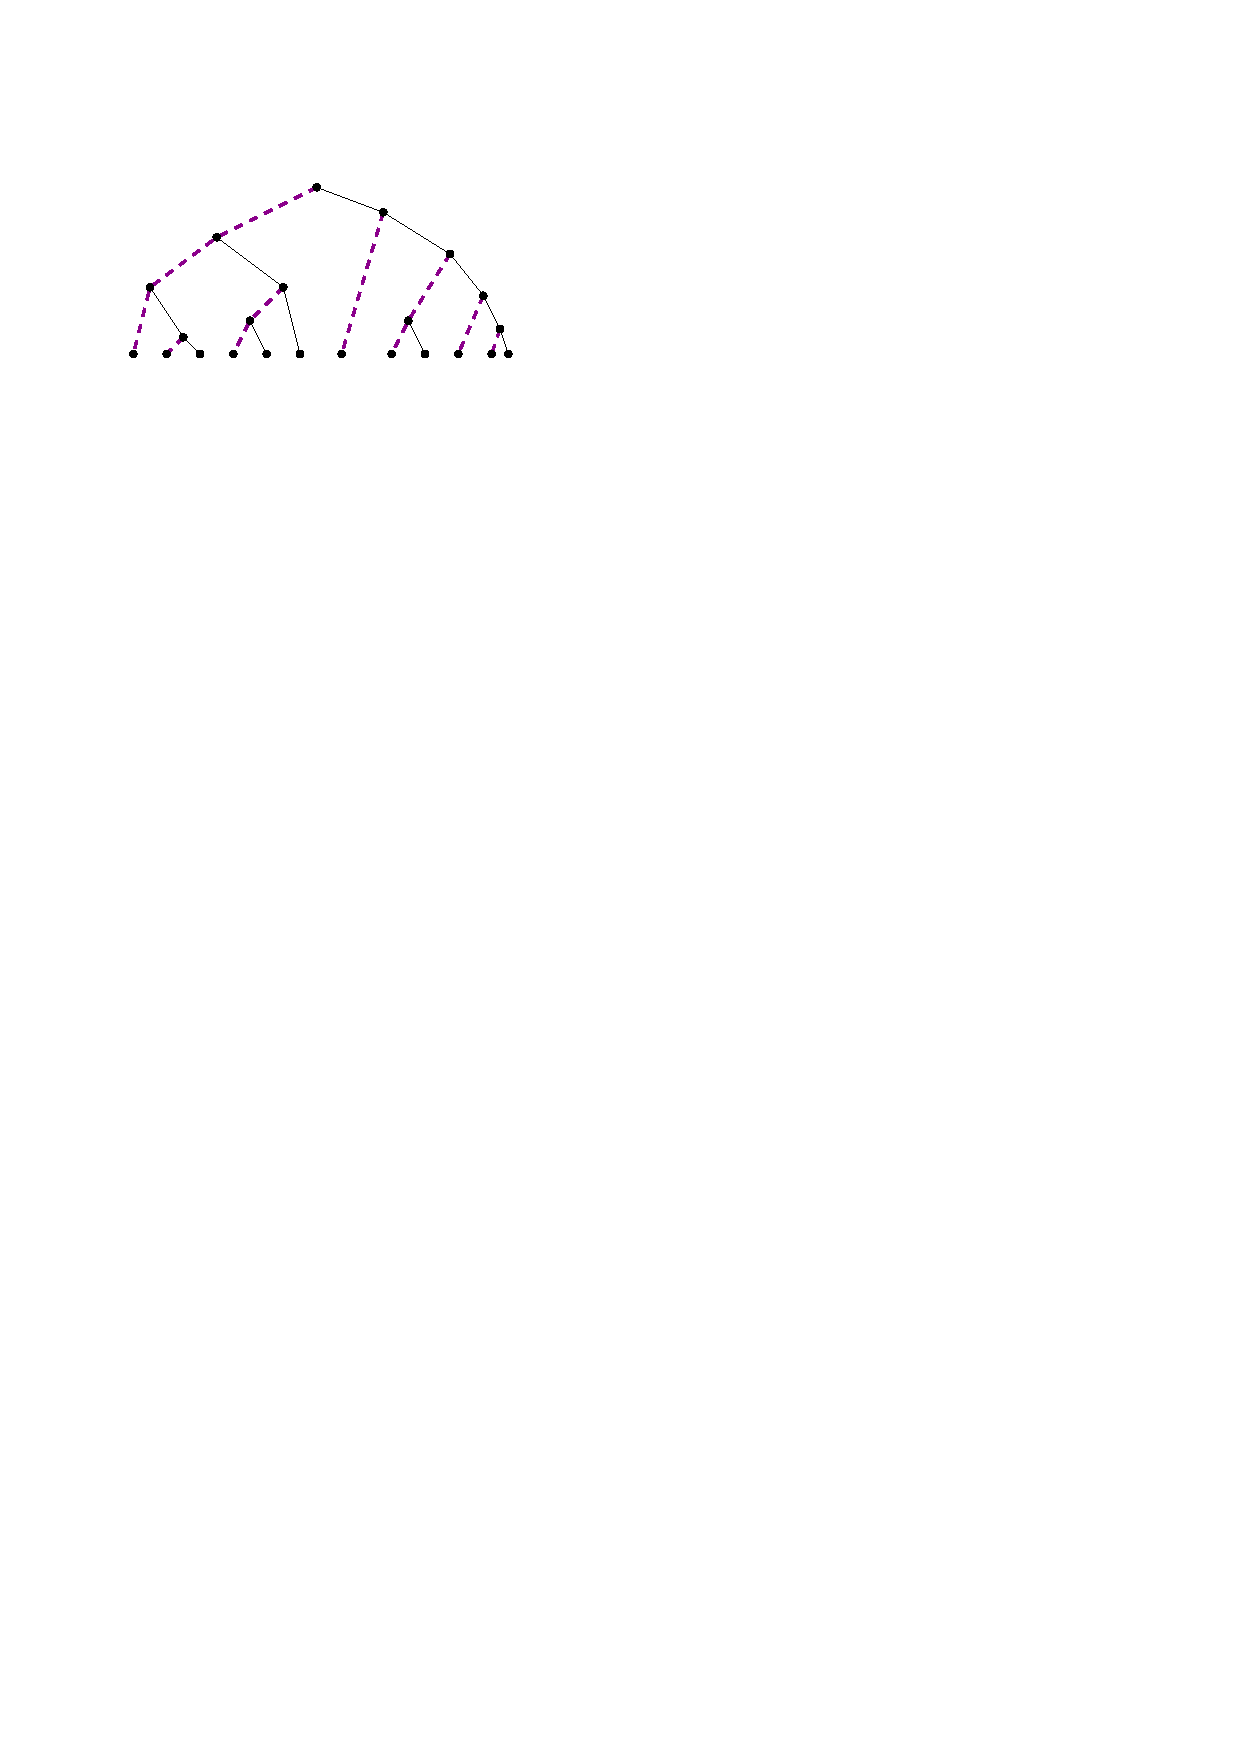
\includegraphics{img/pathdecomp}
\caption{For each leaf $v'$ of $T$, the nodes
$v \in T$ for which $v$ is the leftmost leaf in $T_v$
if a subpath of a root-to-leaf path in $T$. Considering these
subpaths for all leaves in $T$, we obtain a \emph{path decomposition}
of $T$ (shown in bold).}
\label{fig:pathdecomp}
\end{figure}
To do this, we observe the following: let $v' \in T$ be 
a leaf in $T$. Then, $v'$ is the leftmost (or rightmost)
leaf in the subtrees of at most $w$ ancestors $v$ of $v'$.
Furthermore, all these nodes form a subpath (more precisely,
a prefix) of the path from $v$ to the root, see Figure~\ref{fig:pathdecomp}.
Hence, if we maintain the nodes of 
this subpath in a concatenable queue data structure
(realized by, e.g., a balanced binary tree)~\cite{PreparateSh85},
we can obtain $O(\log w)$ update and query time
to find the leftmost (or rightmost) element in $T_v$
for each $v \in T$.
However, we need that the update and query time for this
data structure
depend on the height $h_i$ (i.e, the remaining bits) 
of the query node $v$.
Thus, we partition the possible heights
$\{0, 1, \dots, w\}$ of the nodes on a 
subpath into the sets
$T_{-1} = \{0\}$, $T_i =[2^i, 2^{i+1})$, for $i = 0,\dots,\log w-1$, 
and $T_{\log w} = \{w\}$.
Each set is managed by a balanced binary tree, and the 
roots of the trees are linked together. The height of the $i$-th binary 
search tree is $\log |T_i| = O(i)$. Furthermore, if a query node
of height $h$ is given, 
the set $T_{\lfloor \log h \rfloor}$ is responsible for it, see 
Figure~\ref{fig:queryds}.
\begin{figure}
\centering
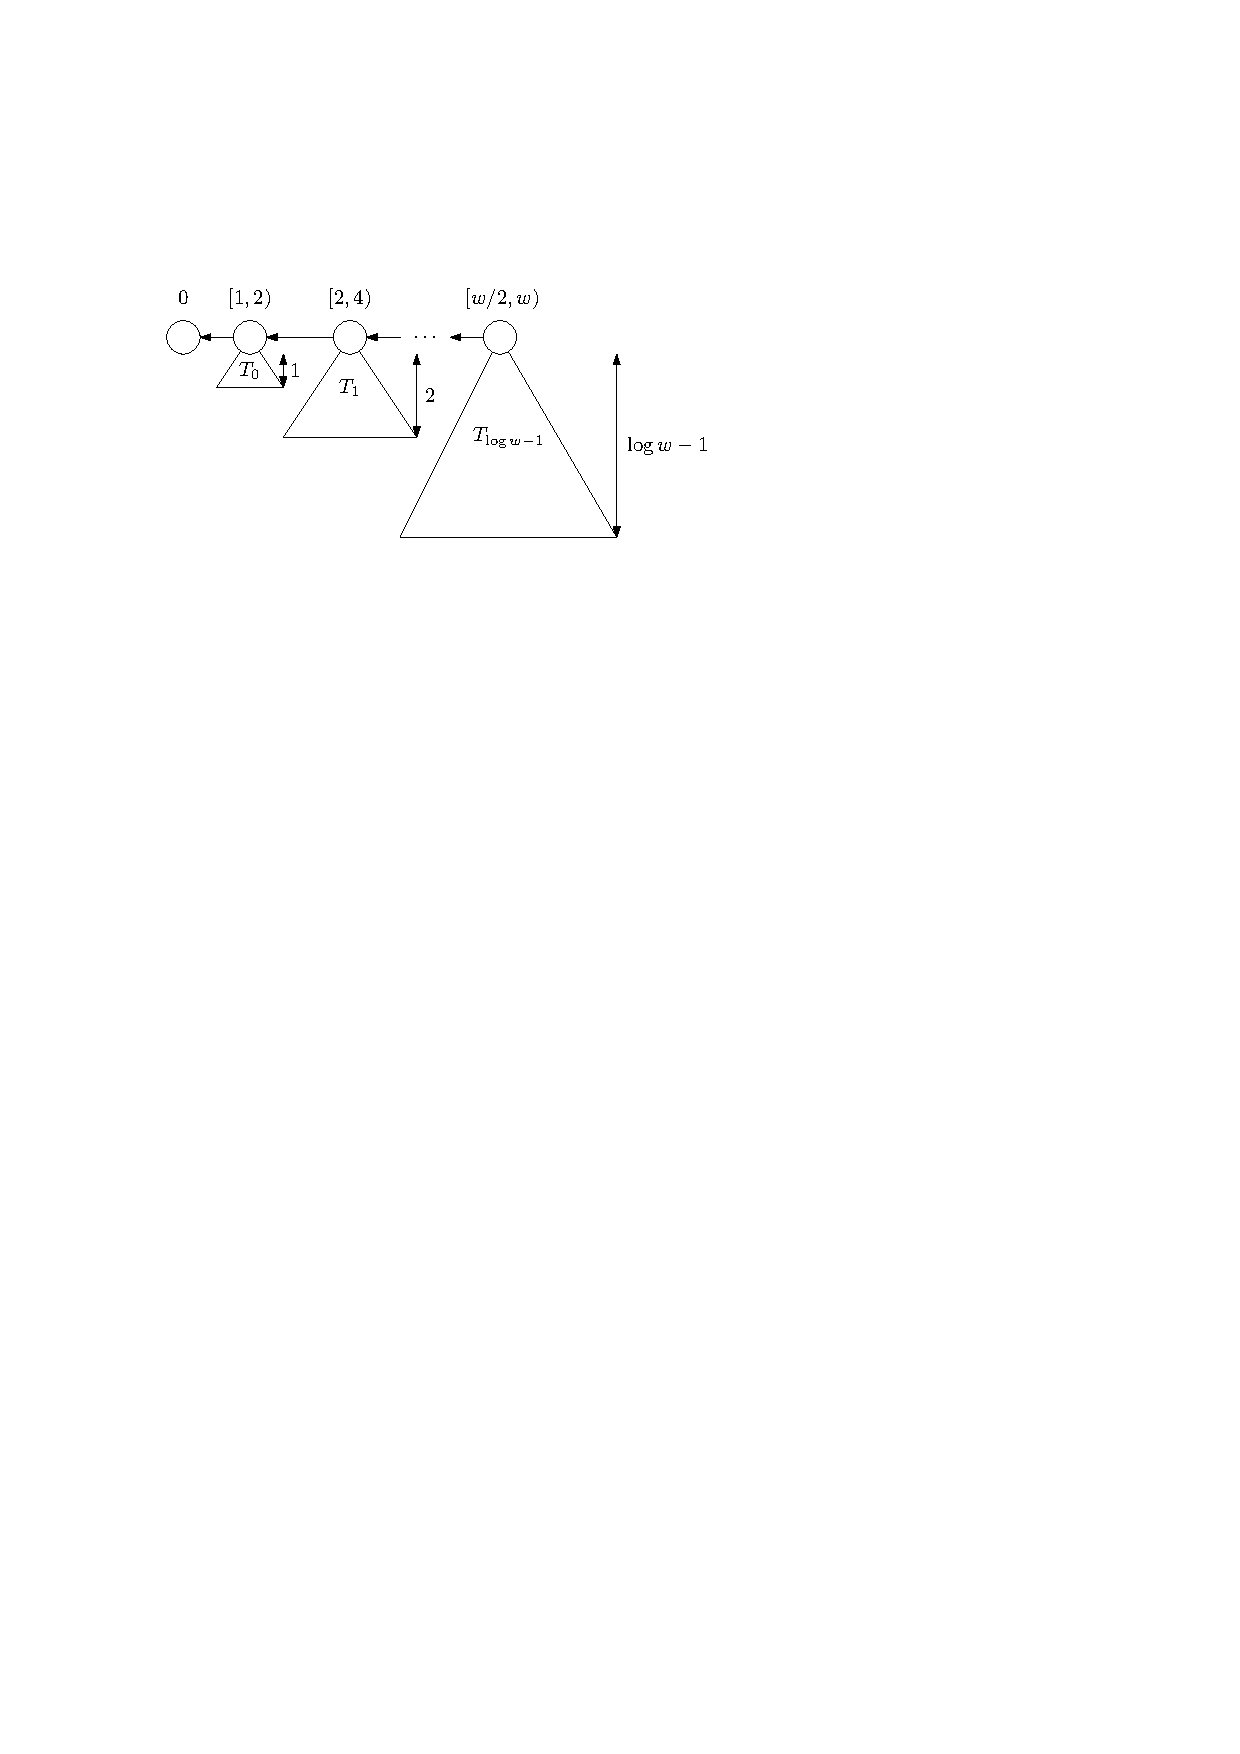
\includegraphics{img/queryds}
\caption{The data structure for a subpath. We group the nodes
in the subpath according to their heights, where the groups
grow exponentially in size. Each group is represented by a
balanced tree. The roots are joined in a linked
list. With this data structure, a node $v$ of height $h$ can
find the leftmost leaf in the subtree $T_v$ in time $O(\log h)$.}
\label{fig:queryds}
\end{figure}


Moreover, $T_{-1}$ is a leaf (the depth of that node is $w$) 
in the trie and therefore the minimum of the whole subpath. Thus, 
the minimum of a subpath can be found from a given node 
$v \in T_i$ in $O(i)$ time by following the
pointers to the root of $T_i$ and the pointers down to $T_{-1}$.

If a node $v$ has $h_k = O(\log \Delta)$ height (remaining bits), 
the node is within
the tree $T_{\lfloor \log h_k \rfloor}$. Thus, it takes 
$O(\log h_k) = O(\log\log\Delta)$ time to find the leftmost
or rightmost leaf in $T_v$.

Furthermore, we can support the following update operations:
(i) \textbf{split}: given a subpath $\pi$ and a node $v$ on $\pi$, split 
the representation of $\pi$ into two representations, one for the 
\emph{lower} subpath from the leaf up to the child of $v$, and
one for the \emph{upper} subpath starting from $v$; and (ii) 
\textbf{join}: given a
representation of an upper subpath starting at a node $v$ obtained 
from an operation of type (i), and a representation for 
a lower subpath up to a child of $v$, join the two representations
into the representation for a joint subpath.
Given the data structure, we can support
both \textbf{split} and \textbf{join} in
 $O(\log h)$ time, where $h$ is the height of 
the node $v$ where the operation occurs. 
This decomposition of $T$ into dynamically changing suppaths
is similar to the \emph{preferred paths decomposition} of
Tango trees~\cite{DemaineHaIaPa07}.

\subsection{Performing an Update}

We know from the Lemma~\ref{lemma:delta_lca_loglog_delta}, that 
the lowest common ancestor of a query element $q$ has expected 
height $h_k = O(\log \Delta)$.

\begin{lemma}
\label{lemma:delta_insert}
Let $S \subseteq U$, and let $T$ be
a randomly shifted $\Delta$-fast tree for 
$S$.  Let $q \in U$ be fixed.
We can insert or delete $q$ into $T$
in $\bigO(\log \log
\Delta)$ expected time, where the expectation is 
over the random choice of the shift $r$.
\end{lemma}

\begin{proof}
To insert $q$ into $T$, we need to split an edge $(u,v)$ of $T$ into
two edges $(u,b)$ and $(b,v)$. This creates
exactly two new nodes in $T$, an inner node and a leaf node. 
The branch node is exactly $\lca_T(q)$, and it has expected height 
$h_k = O(\log \Delta)$, by Lemma~\ref{lemma:delta_lca_loglog_delta}. 
Thus, it will
take $O(\log\log \Delta)$ expected time to find
the edge $(u,v)$, by
Corollary~\ref{cor:delta_fast_expected_lca}.

Once the edge $(u,v)$ is found, the hash maps $H_z$ and $H_u$ 
can then be updated in constant time.
Now let us consider the update time of the 
hash map $H_\Delta$. Recall that
$H_\Delta$ stores the lowest branch nodes for all prefixes
of the elements in $S$ that have certain lengths.
This means that all prefixes on the edge $(b,v)$ which 
are stored in the hash map $T_\Delta$ need to
be updated. Furthermore, prefixes at certain depths which 
are on the new edge $(b,q)$ need to
be added. For the edge $(b,v)$, we will enumerate 
all prefixes at certain depths, but we will select only those that 
lie on the edge $(b,v)$. This needs
$O(\log\log\log\Delta)$ insertions and updates in total: we
have to insert the prefixes $q_0 \dots q_{d_i}$ for all 
$i \geq 1$ with $d_i < |b|$. Since we defined 
$d_i = w - h_i = w - 2^{2^i}$, 
and since $|b| = w - O(\log \Delta)$, 
we have that $d_i \leq |b|$ as soon as 
$c \log\Delta < 2^{2^i}$. This holds for 
$i > \log\log (c\log \Delta)$, and hence $i =
\Theta(\log\log\log\Delta)$.

After that, the leftmost and rightmost elements for the subtrees
of $T$ have to be updated. For this, we need to add one
subpath for the new leaf $q$, and we may need to split
a subpath at a node of height $h_k = O(\log \Delta)$ and join
the resulting upper path with the newly created subpath. As we
have seen, this takes $O(\log h_k) = O(\log \log \Delta)$ time.

The operations for deleting an element $q$ from $S$ are symmetric.
\end{proof}

The following theorem summarizes our result.

\begin{theorem}
Let $r \in U$ be picked uniformly at random.
After performing a shift of $U$ by $r$, 
the $\Delta$-fast trie provides a data structure for the
dynamic predecessor problem such that the 
query operations take $O(\log \log \Delta)$ worst-case time and 
the update operations need $O(\log \log \Delta)$ expected
time, for $\Delta = \min \{|q-q^+|, |q-q^-|\}$, where $q$ is the
requested element and $q^+$ and $q^-$ are the predecessor and
successor of $q$ in the current set $S$. At any point in time, 
the data structure needs $O(n)$ words of space, where $n = |S|$.
\end{theorem}

\section{Applications}

Bose~\etal~\cite{BoseDoDuHoMo13} describe how to combine their structure
with a technique of Chan~\cite{Chan02} and random 
shifting~\cite[Chapter~11]{HarPeled11} for obtaining a data structure for 
distance-sensitive
approximate nearest neighbor queries on a grid.
More precisely, let $d \in \N$ be the fixed dimension, 
$U = \{0, \dots, 2^{w}-1\}$ be the universe, and
let $\eps > 0$ be given.
The goal is to maintain a dynamic set $S \subseteq U^d$ under
insertions, deletions, and \emph{$\eps$-approximate
nearest neighbor queries}: given a query point $q \in U^d$,
find a $p \in S$ with $d_2(p,q) \leq (1+\eps)d_2(p, S)$.
Plugging our $\Delta$-fast tries into the structure of
Bose~\etal~\cite[Theorem~9]{BoseDoDuHoMo13}, we can
immediately improve the space requirement of their structure to linear:
\begin{theorem}
Let $U = \{0, \dots, 2^w-1\}$ and let $d$ be a constant.
Furthermore, let $\eps > 0$ be given.
There exists a data structure that supports $(1+\eps)$-approximate
nearest neighbor queries over a subset $S \subseteq U^d$ in 
$(1/\eps^d)\log\log \Delta)$ expected time and insertions and deletions
of elements of $U^d$ in $O(\log\log \Delta)$ expected time.
Here, $\Delta$ denotes the Euclidean distance between the query element
and $S$. At any point in time, the data structure requires $O(n)$
words of space, where $n  = |S|$.
\end{theorem}

As a second application, Bose~\etal~\cite{BoseDoDuHoMo13}
present a data structure for dominance queries on a grid,
based on a technique of Overmars~\cite{Overmars88}.
Again, let $U = \{0, \dots, 2^w-1\}$, and let $S \subseteq U^2$,
$|S| = n$ be given. The goal is to construct a data structure
for \emph{dominance queries} in $S$. That is, given a query point
$q \in U^2$, find all points $p$ in $S$ that \emph{dominate} $q$,
i.e., for which we have $p_x \geq q_x$ and $p_y \geq q_y$, there
$p_x$, $p_y$ and $q_x$, $q_y$ are the $x$- and $y$-coordinates 
of $p$ and $q$.

Again, using $\Delta$-fast tries, we can immediately improve the
space requirement for the result of 
Bose~\etal~\cite[Theorem~10, Corollary~13]{BoseDoDuHoMo13}.

\begin{theorem}
Let $U = \{0, \dots, 2^w-1\}$, and let $S \subseteq U^2$, $|S|=n$
be given. There exists a data structure that reports the points in $S$
that dominate a given query point $q = (a,b) \in U^2$ in expected time
$O(\log\log(h+v) + k)$, where $h = 2^w - a$, $v = 2^2-b$, and $k$
is the number of points in $S$ dominated by $q$.
The data structure uses $O(n \log n)$ space.
\end{theorem}
\section{Conclusion}

We present a new data structure for local searches
in bounded universes. This structure now interpolates
seamlessly between hashtables and van-Emde-Boas trees,
while requiring only a linear number of words. This provides
an improved, and in our opinion also slightly simpler, version
of a data structure by Bose \etal~\cite{BoseDoDuHoMo13}.
All the operations of our structure can be
presented explicitly in pseudocode. This can be found in the
Master's thesis of the first author~\cite{Ehrhardt15}.

\bigskip
\noindent\textbf{Acknowledgments.}
We thank the anonymous reviewers for numerous
insightful comments that improved the quality of the paper.
In particular, we would like to thank the anonymous 
reviewers for pointing us to~\cite{BelazzougiBoVi12}.
\bibliographystyle{splncs03}
\bibliography{delta_fast}
\end{document}

